\documentclass[11pt,a4paper]{article}

\usepackage[margin=1in]{geometry}
\usepackage[T1]{fontenc}
\usepackage[utf8]{inputenc}
\usepackage{lmodern}
\usepackage{hyperref}
\usepackage{graphicx}
\usepackage{amsmath,amssymb}
\usepackage{booktabs}
\usepackage{array}
\usepackage{tabularx}
\usepackage{float}
\title{LLM Inference Documentation}
\author{Moritz Anton Zideck}
\date{\today}

\begin{document}

\maketitle

\tableofcontents
\newpage

\section{Introduction}
In this submission a performance analysis of LLM Inference Engines should be done.
The main goal hierby is to find limitations and optimization during CPU-Inference.
Since we run on the CPU limitations include memory bandwidth, therefore feeding the CPU cores fast enough with data so they can work most efficient as well as variable thread count.
For all of the tests a llama.cpp engine is used since it already supports the common gguf file nativly and is fast to set up and run.
To get a deeper insight the behaviour of model inference the Track A has been chosen using the same model with different setups.

\section{Background}
The most common problem in CPU inference is not getting the data fast enough to the CPU.
This means the model weights needed for calculation are supplied slower than they are used to generate output tokens.
Therefore, many optimisations try to tackle exactly this, with a well-known example being quantisation.
It is used to reduce the model size by representing each weight with a lower number of bits.
Tests showed that going from 16 bits per weight to 8 bits reduces the model size by 50\%, while the precision loss is only minor.
Another important technique is the KV cache, which is used during autoregressive generation.
Instead of recalculating the key and value vectors for all previous tokens every time a new token is generated, the system stores them and reuses them in the next step.
This greatly reduces repeated computation, especially for longer prompts, but it also introduces a new memory cost because the cache grows with the sequence length.
On CPUs, this can again become limited by memory bandwidth, so the cache has to be managed efficiently.
Threading is also important because CPUs usually have multiple cores that can work in parallel.
Matrix multiplications and other operations can be split across threads, which improves speed, but only up to the point where the memory system becomes saturated or the overhead of coordinating threads becomes too large.
Finally, batching can improve throughput by processing multiple requests or tokens together. This allows the same model weights to be reused more efficiently once they are loaded into cache or memory.
However, batching also increases latency for individual users, because requests may have to wait until a batch is formed.
In a CPU-only inference system, the best performance therefore comes from combining these techniques carefully: quantisation reduces the amount of data that must be moved, the KV cache avoids unnecessary recomputation, threading uses the available cores, and batching improves weight reuse without making latency too high.

\section{Methodology}
For the evaluation the Deucalion Supercomputer is used.
The Performance model pipeline training were run on the ARM Partition using a FUJITSU A64FX with 48 Cores as well 32GB of RAM.
Custom Tests peaked at 1.9T FLOPS with a C matrix mulitplication script as well as a DRAM Bandwidth of 450 GB/S.
The inference llama.cpp engine version llama.cpp/20260415-foss-2023a  build with GNU 12.3.0 for Linux aarch64.
For the Track A model deepdive pipeline the training was run on the x86 partinion using a AMD EPYC 7742 64-Core Processor with 128 threads as well as 256GB RAM.
A custom inference setup was created with AI to test different configuration at once with in depth result gathering while keeping the the static paramters unchanged.
For final result evaluation Jupyter Notebooks are used to parse and visualise results.
\subsection{Performance model pipeline}
To determine the precision of the performance model, the \texttt{llama-bench} command is used.
For a given model, thread count, number of prompt tokens, and number of generated tokens,
\texttt{llama-bench} reports both the prompt processing throughput in prompt tokens per second and
the generation throughput in tokens per second.

All benchmark experiments were conducted on a Deucalion ARM node with the following measured hardware characteristics:
\begin{itemize}
    \item Measured TFLOPs: 1.9T
    \item Measured Memory Bandwidth: 450 GB/s
\end{itemize}

The inference engine \texttt{llama.cpp} with 48 threads was used for all tests.
This setup is executed through a custom shell script, which samples three different models,
as described in Section~4. During the benchmark runs, the number of threads, the number of
prompt tokens, and the number of generated tokens are varied.

The resulting measurements are stored in a JSON file. This file is then read by a Jupyter
notebook, which is used to generate the final results and visualizations.
\subsection{Track A model deepdive pipeline}
For the model deep dive, the model gemma-2-2b-it-Q4\_K\_M is used. This is a compact, instruction-tuned Gemma 2B-class model packaged as a GGUF file and quantized with Q4\_K\_M.
The quantized variant reduces memory footprint and bandwidth pressure while keeping representative instruction-following behavior, which makes it well suited for CPU-only profiling.
Its smaller size also allows wider sweeps across prompt length, generation length, and threading without exceeding memory limits.
The \texttt{llama-cli} is used so that real prompts can be processed and generated. To support this, a sophisticated benchmark pipeline was created with the help of AI.
For each model, four major configuration groups are tested:
\begin{enumerate}
    \item \textbf{Threading / concurrency}
    \begin{itemize}
        \item Thread counts: 4, 16, 64, and 128
        \item Multiple concurrent requests are sent at the same time, using concurrency levels of 2, 4, and 16
    \end{itemize}

    \item \textbf{Prompt length}
    \begin{itemize}
        \item Prompt lengths: 32, 128, 512, and 2048 tokens
    \end{itemize}

    \item \textbf{Generation length}
    \begin{itemize}
        \item Generation lengths: 32, 128, 512, and 2048 tokens
    \end{itemize}

    \item \textbf{Fixed-thread baseline runs}
    \begin{itemize}
        \item Except for the threading experiments, all other runs are executed with 16 threads.
    \end{itemize}
\end{enumerate}
For every configuration, all 30 prompts are executed three times. The benchmark produces a comprehensive result file containing detailed runtime information, including generation token timestamps, prompt processing time, generation time, requests, and responses.
This result file is then parsed to generate a complete CSV containing all required metrics, such as TTFT, TOPT, mean values, and standard deviations. These CSV files are subsequently used to create the final result visualizations.

\section{Analytical Model Proposal}
\label{sec:analytical-model-proposal}
Two import key metrices are:
\begin{itemize}
    \item \textbf{TTFT (Time to First Token):} The total time from sending a request to receiving the first generated token, including prompt processing and the first decode step.
    \item \textbf{TPOT (Time Per Output Token):} The average time to generate each subsequent token after the first token, measured during steady-state generation.
\end{itemize}

\subsection{TTFT Assumption}
Similar to the TPOT Assumption a TTFT Assumption can be made using computing paramters from our system.
Since the available cache capacity is much smaller than the model weights, weight reuse from cache can be neglected. The test will also be done with a smaller model to see the impact of the cache.
To create the first token, two phases must be taken into account:
\begin{itemize}
    \item \textbf{Prefill Phase:} Processing of input tokens
    \item \textbf{Generation Phase:} Generating output
\end{itemize}
In the prefill phase, the model weights must be read once from memory while the entire prompt is processed in parallel. Therefore, the prefill latency is the maximum of the memory-transfer time and the compute time for all prompt tokens:
\begin{equation}
T_{\text{prefill}} = \max\left(
    \frac{\text{Model Size}}{\text{Memory Bandwidth}},
    \frac{2 \times \text{Prompt Length} \times \text{Parameters}}{\text{Effective TFLOPs}}
\right)
\end{equation}
The factor of 2 appears because each parameter participates in one multiply-accumulate (MAC) operation, which corresponds to two floating-point operations (one multiply and one add).
To generate the first output token, the model weights are read once again and a single forward pass is executed. The latency of this decode step is:
\begin{equation}
T_{\text{first token}} = \max\left(
    \frac{\text{Model Size}}{\text{Memory Bandwidth}},
    \frac{2 \times \text{Parameters}}{\text{Effective TFLOPs}}
\right)
\end{equation}
The Time to First Token (TTFT) is the sum of the prefill time and the first-token decode time:
\begin{equation}
\text{TTFT} = T_{\text{prefill}} + T_{\text{first token}}
\end{equation}
\subsection{Models Tested}
\label{sec:models}
\begin{itemize}
    \item \textbf{Meta-Llama-3.1-8B-Instruct-Q4\_K\_M}
    \begin{itemize}
        \item Model size: 4.5 GB
        \item Parameters: 8 Billion
        \item Formula: $\text{TTFT} = \max(0.0100, 0.008421L) + 0.0100$
    \end{itemize}
    \item \textbf{Gemma-2-2b-it-Q8\_0}
    \begin{itemize}
        \item Model size: 2.6 GB
        \item Parameters: 2.6 Billion
        \item Formula: $\text{TTFT} = \max(0.00578, 0.002737L) + 0.00578$
    \end{itemize}
    \item \textbf{SmolLM2-1.7B-Instruct-Q4\_K\_M}
    \begin{itemize}
        \item Model size: 1 GB
        \item Parameters: 1.7 Billion
        \item Formula: $\text{TTFT} = \max(0.00222, 0.001789L) + 0.00222$
    \end{itemize}
\end{itemize}
where L is the prompt length.

\section{Results}
This section reports results from the model pipeline benchmarks and the model deepdive runs. Figures are shown inline, and detailed tables are collected in Appendix \ref{sec:appendix_results_tables}.

\subsection{Calculated TTFT Results}
Measured and predicted TTFT values were collected for three models across prompt lengths used in the pipeline benchmarks. The full numeric results are listed in Table \ref{tab:ttft_predicted_measured} in Appendix \ref{sec:appendix_results_tables}.
\begin{table}[H]
\centering
\small
\setlength{\tabcolsep}{4pt}
\begin{tabularx}{\textwidth}{X|c|c|c}
    \toprule
    Model & Prompt Length & Predicted TTFT (ms) & Measured TTFT (ms) \\
    \midrule
    Meta-Llama-3.1-8B-Instruct-Q4\_K\_M & 32   & 280   & 9406  \\
    Meta-Llama-3.1-8B-Instruct-Q4\_K\_M & 128  & 1088  & 11760 \\
    Meta-Llama-3.1-8B-Instruct-Q4\_K\_M & 512  & 4321  & 16680 \\
    Meta-Llama-3.1-8B-Instruct-Q4\_K\_M & 2048 & 17257 & 75260 \\
    Meta-Llama-3.1-8B-Instruct-Q4\_K\_M & 8192 & 68986 & --    \\
    \midrule
    Gemma-2-2b-it-Q8\_0 & 32   & 93    & 2873  \\
    Gemma-2-2b-it-Q8\_0 & 128  & 356   & 3558  \\
    Gemma-2-2b-it-Q8\_0 & 512  & 1407  & 5153  \\
    Gemma-2-2b-it-Q8\_0 & 2048 & 5611  & 23890 \\
    Gemma-2-2b-it-Q8\_0 & 8192 & 22429 & --    \\
    \midrule
    SmolLM2-1.7B-Instruct-Q4\_K\_M & 32   & 59    & 1328 \\
    SmolLM2-1.7B-Instruct-Q4\_K\_M & 128  & 231   & 1433 \\
    SmolLM2-1.7B-Instruct-Q4\_K\_M & 512  & 918   & 1775 \\
    SmolLM2-1.7B-Instruct-Q4\_K\_M & 2048 & 3665  & 8654 \\
    SmolLM2-1.7B-Instruct-Q4\_K\_M & 8192 & 14657 & --   \\
    \bottomrule
\end{tabularx}
\caption{Predicted and measured TTFT results for different models and prompt lengths.}
\label{tab:ttft_predicted_measured}
\end{table}
The figure below shows the measured TTFT values across prompt lengths for the same runs.
\begin{figure}[H]
\centering
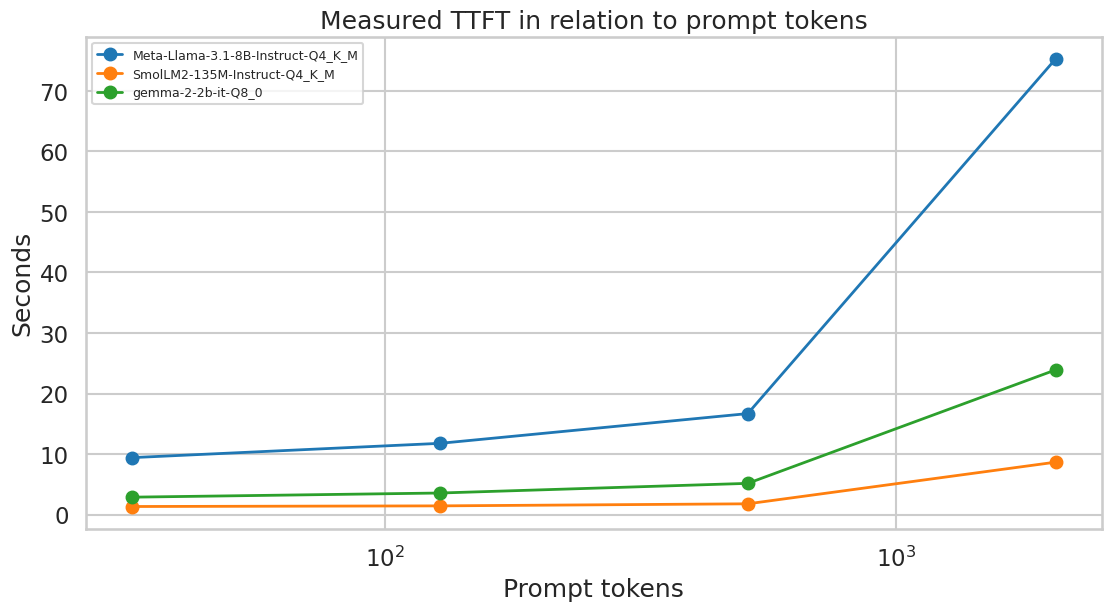
\includegraphics[width=\textwidth]{plots/model_pipeline/ttft.png}
\caption{TTFT measurements for the model pipeline benchmarks.}
\label{fig:model_pipeline_ttft}
\end{figure}
\subsection{Model Comparison}
\subsubsection{Summary Metrics}
Table \ref{tab:model_performance_summary} in Appendix \ref{sec:appendix_results_tables} lists TTFT at 128 tokens, TPOT, and throughput for prefill and generation for each model.

\subsubsection{Thread Scaling}
The thread scaling plot presents benchmark measurements across different thread counts.
\begin{figure}[H]
\centering
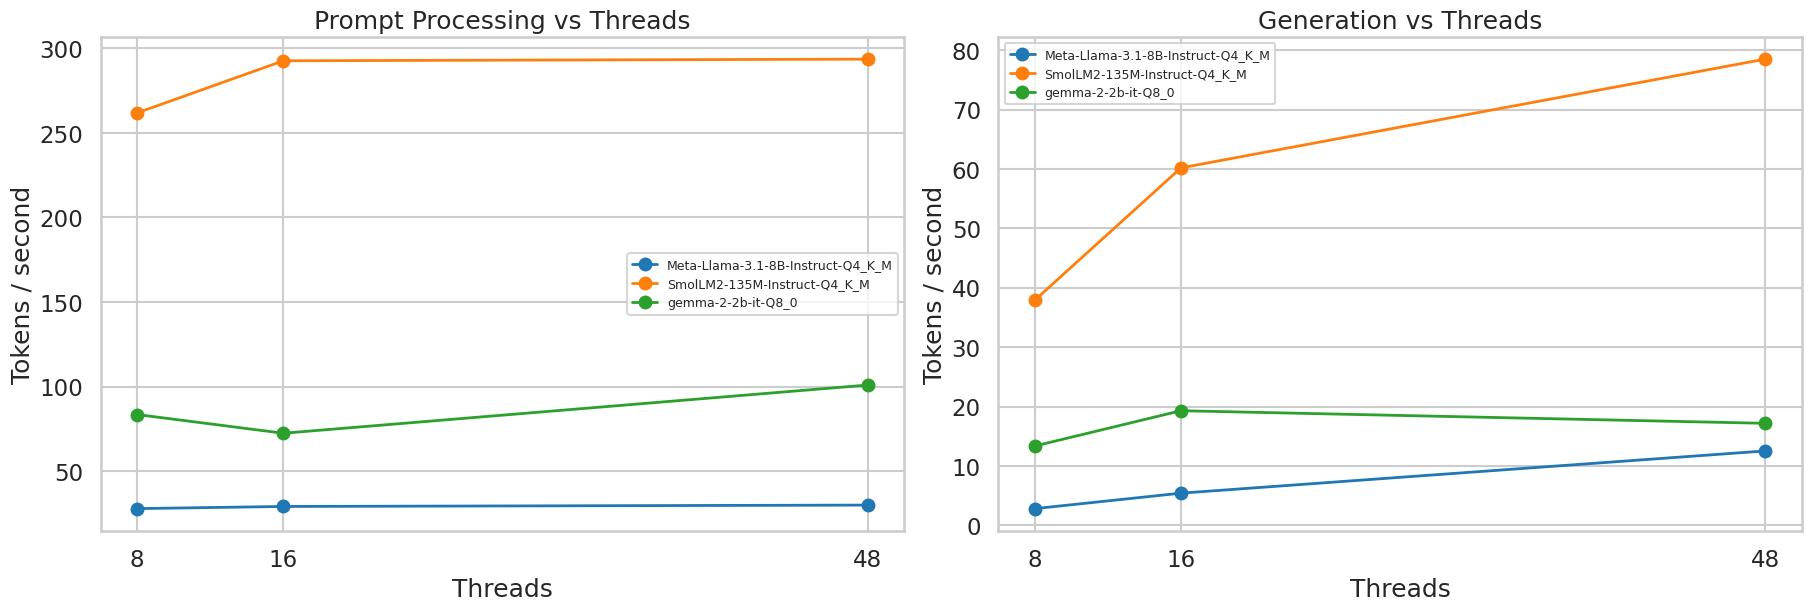
\includegraphics[width=\textwidth]{plots/model_pipeline/threads.png}
\caption{Thread scaling results from the model pipeline benchmarks.}
\label{fig:model_pipeline_threads}
\end{figure}

\subsubsection{Throughput}
The throughput plot shows prompt processing and generation rates across the tested configurations.
\begin{figure}[H]
\centering
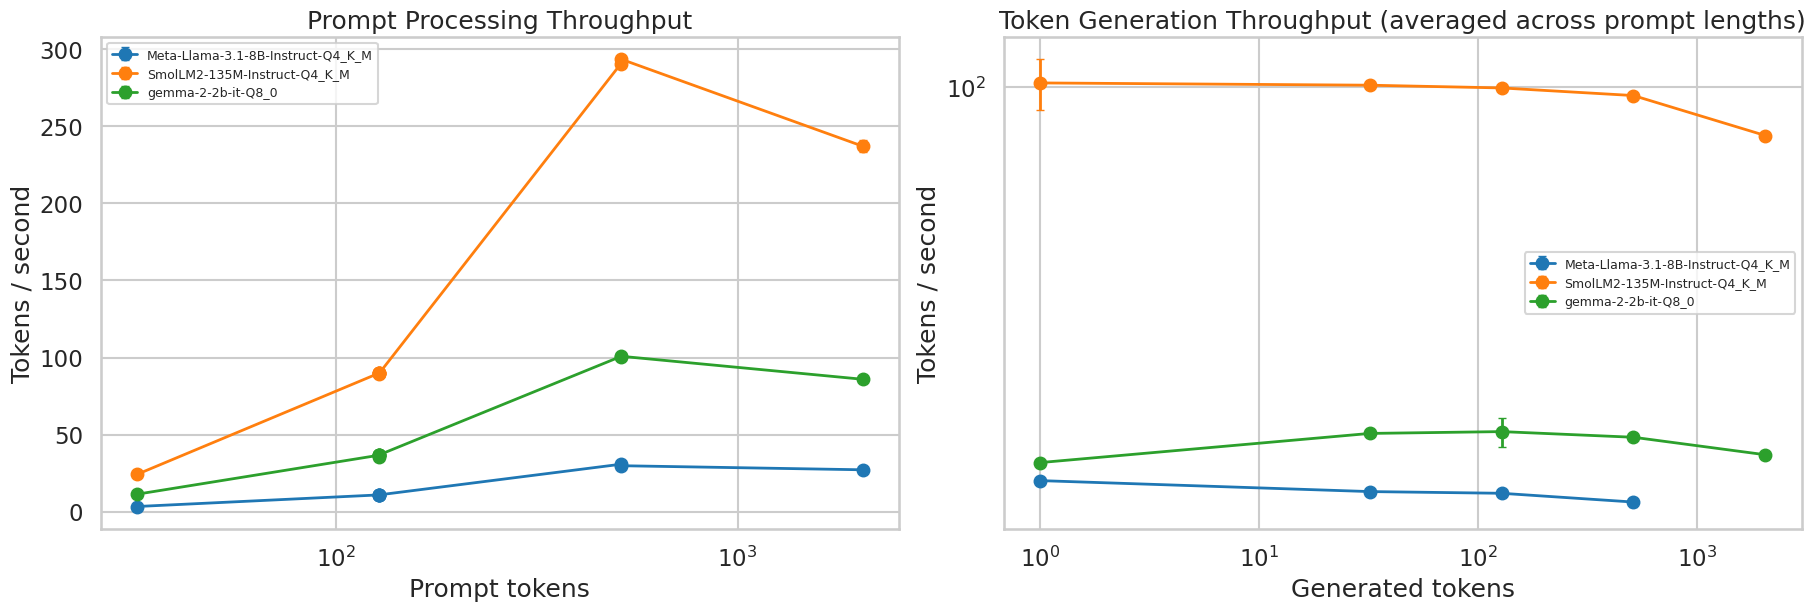
\includegraphics[width=\textwidth]{plots/model_pipeline/throughput.png}
\caption{Throughput measurements for the model pipeline benchmarks.}
\label{fig:model_pipeline_throughput}
\end{figure}
\subsection{Model deepdive - Gemma-2-2b-it-Q4}
This deepdive focuses on a single model to isolate how CPU inference responds to thread count, concurrency, prompt length, and decode length. By separating prompt processing (prefill) from token generation, it highlights how these phases scale differently under the same hardware and model constraints. Detailed tables are provided in Appendix \ref{sec:appendix_results_tables}.

\subsubsection{Thread Count and Memory Usage}
Table \ref{tab:model_deepdive_summary} lists TTFT, TPOT, and memory usage for thread configurations and prompt categories.
The figure below shows processing and generation time versus thread count.

\begin{figure}[H]
\centering
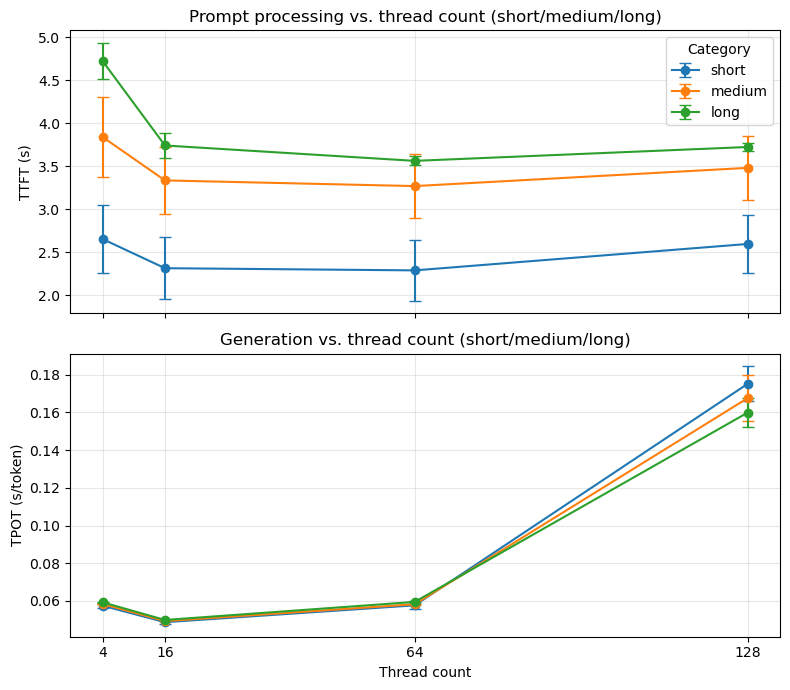
\includegraphics[width=\textwidth]{plots/model_deepdive/processing-generation-vs-thread-count.png}
\caption{Processing and generation time versus thread count in the model deepdive.}
\label{fig:model_deepdive_processing_generation_threads}
\end{figure}

The figure below shows memory usage versus thread count.
\begin{figure}[H]
\centering
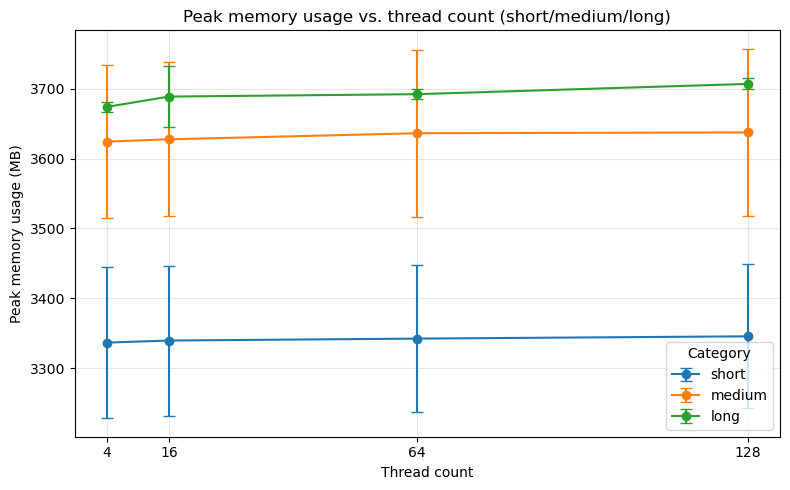
\includegraphics[width=\textwidth]{plots/model_deepdive/memory-usage-vs-thread-count.png}
\caption{Memory usage versus thread count in the model deepdive.}
\label{fig:model_deepdive_memory_usage_threads}
\end{figure}

\subsubsection{Concurrency Throughput}
Concurrency tests use multiple workers sending concurrent requests to the CPU, with each worker configured to use 4 threads. This setup tests how CPU processing behaves when multiple requests happen at the same time. The 16-worker run was too slow and was canceled, so only a short measurement is available.
Table \ref{tab:model_deepdive_concurrency_throughput} reports generation and prompt throughput for concurrency levels and prompt categories.
The figure below shows generation throughput versus concurrency.

\begin{figure}[H]
\centering
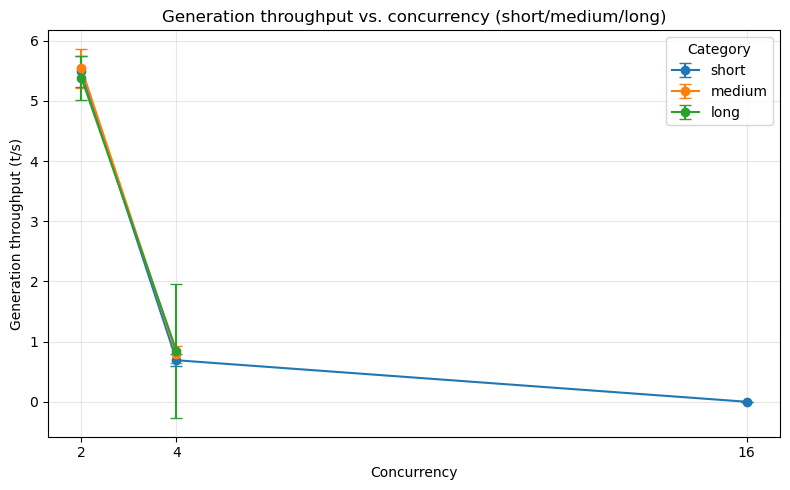
\includegraphics[width=\textwidth]{plots/model_deepdive/generation-vs-concurrency.png}
\caption{Generation throughput versus concurrency in the model deepdive.}
\label{fig:model_deepdive_generation_vs_concurrency}
\end{figure}

The figure below shows prompt processing throughput versus concurrency.
\begin{figure}[H]
\centering
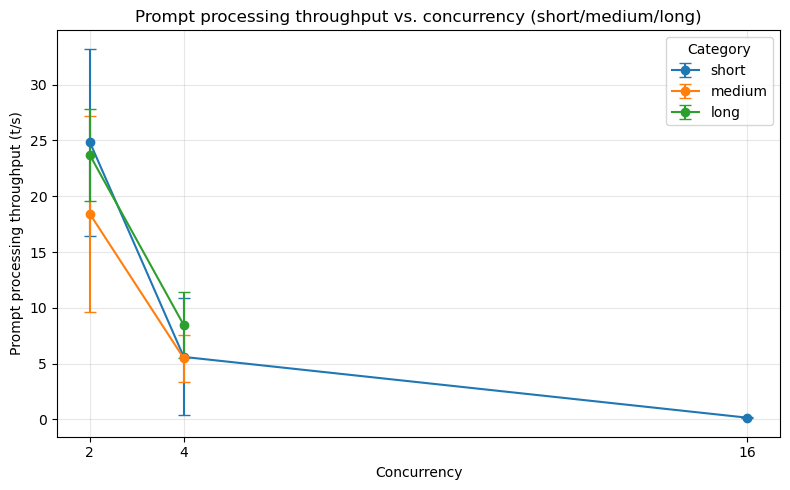
\includegraphics[width=\textwidth]{plots/model_deepdive/processing-vs-concurrency.png}
\caption{Prompt processing throughput versus concurrency in the model deepdive.}
\label{fig:model_deepdive_processing_vs_concurrency}
\end{figure}

\subsubsection{Context Length}
Table \ref{tab:model_deepdive_ttft_context_length} summarizes TTFT by context length.
The figure below shows TTFT versus prompt length.

\begin{figure}[H]
\centering
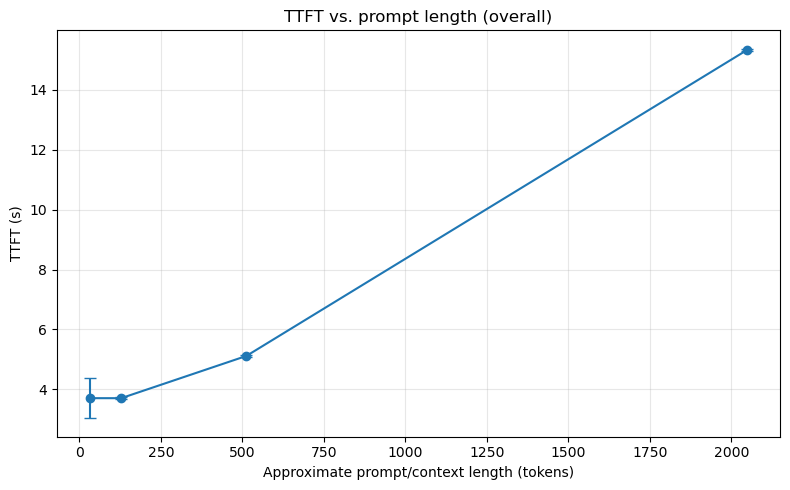
\includegraphics[width=\textwidth]{plots/model_deepdive/ttft-vs-promt-length.png}
\caption{TTFT versus prompt length in the model deepdive.}
\label{fig:model_deepdive_ttft_vs_prompt_length}
\end{figure}

\subsubsection{TPOT Baseline and Measured TPOT}
On CPUs, TPOT is often limited more by memory bandwidth than by compute. A simple way to capture this is to treat each token as a model-size read from DRAM, which gives a constant, bandwidth-bound prediction:
\begin{equation}
TPOT_{pred} = \frac{\text{model\_size\_MB}}{\text{DRAM\_bandwidth\_MB/s}}
\end{equation}
Using DRAM bandwidth MB/s = 280GB/s and model size = 1.7 GB, the prediction is a straight horizontal line. The plots below compare that baseline with measured TPOT across thread count and decode length, split into short/medium/long categories.

Table \ref{tab:model_deepdive_tpot_thread_count} lists observed TPOT by thread count and category, and Table \ref{tab:model_deepdive_tpot_decode_length} lists observed TPOT by decode length and category.

\begin{figure}[H]
\centering
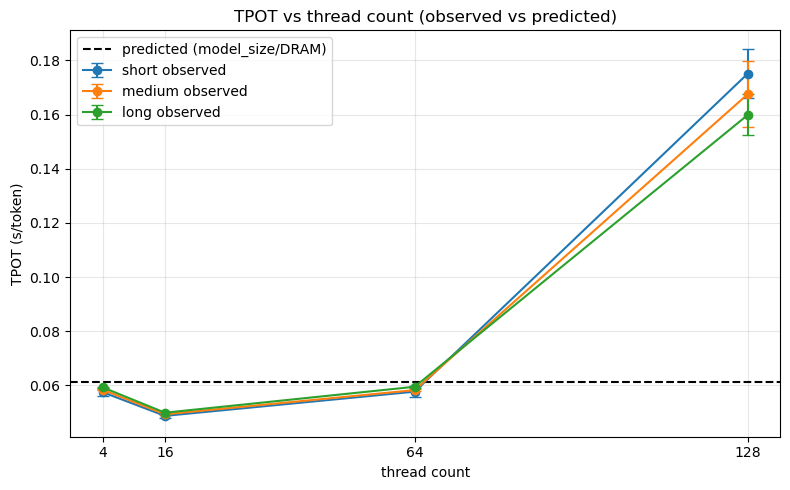
\includegraphics[width=\textwidth]{plots/model_deepdive/tpot-vs-thread-count.png}
\caption{Observed TPOT versus thread count in the model deepdive.}
\label{fig:model_deepdive_tpot_vs_thread_count}
\end{figure}

\begin{figure}[H]
\centering
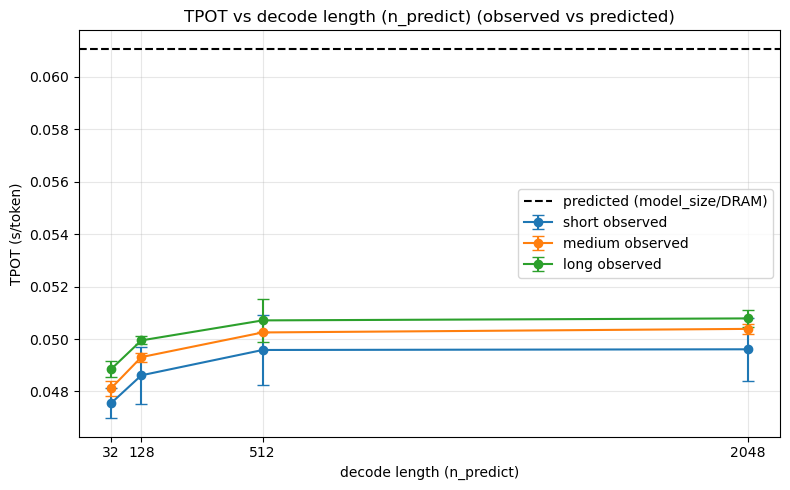
\includegraphics[width=\textwidth]{plots/model_deepdive/tpot-vs-decode-length.png}
\caption{Observed TPOT versus decode length in the model deepdive.}
\label{fig:model_deepdive_tpot_vs_decode_length}
\end{figure}

\section{Discussion}

\subsection*{Model Comparison and Threading}
For larger models that are memory bound, increasing core count does not show measurable improvement because performance is limited by memory bandwidth.
For a smaller model such as SmolLM2, which is not memory bound, larger performance gains are observed when using more cores.

\subsection*{Prompt and Generation Length Effects}
Across the tested models, performance remains mostly stable over different prompt lengths and generation lengths.
The best processing performance is observed at a prompt length of 512 tokens, while a slight dip appears at high generation lengths around 2048 tokens.

\subsection*{Model Deepdive Findings}
The model deepdive shows that prompt processing and token generation scale differently, indicating distinct computation phases (Fig.~\ref{fig:model_deepdive_processing_generation_threads}).
In the processing phase, additional threads reduce latency up to roughly 16--32 threads, after which improvements taper; performance degrades at 128 threads, which is consistent with thread management and synchronization overhead dominating the gains (Fig.~\ref{fig:model_deepdive_processing_generation_threads}).
In contrast, generation is dominated by per-token weight reads rather than prompt processing, and higher thread counts harm generation throughput; the 128-thread case is roughly 3x slower than 16 threads, showing that more parallelism cannot hide the memory cost of decoding (Fig.~\ref{fig:model_deepdive_processing_generation_threads}).
Concurrency further stresses the system: throughput drops sharply beyond 4 concurrent requests, and the 16-request run was too slow to complete and was canceled (Fig.~\ref{fig:model_deepdive_generation_vs_concurrency}, Fig.~\ref{fig:model_deepdive_processing_vs_concurrency}).
TTFT scales approximately linearly with prompt length, while short prompts show a visible fixed overhead that raises the per-token cost (Fig.~\ref{fig:model_deepdive_ttft_vs_prompt_length}).
Finally, the measured TPOT at 16 threads tracks the memory-bandwidth prediction closely, supporting the bandwidth-bound assumption used for CPU inference modeling (Fig.~\ref{fig:model_deepdive_tpot_vs_thread_count}).

\subsection*{Analytical Model Considerations}
The real implementation introduces significant overhead, which is most visible at low prompt lengths.
In the analytical model, we use a measured performance of 1.9 TFLOPs, obtained from a C-based matrix multiplication benchmark using all cores.
However, this value does not necessarily represent the effective TFLOPs achieved during LLM inference.
For a more precise model, both the implementation overhead and the actual inference TFLOPs would need to be measured.
Nevertheless, the model provides a useful general direction for understanding how TTFT behaves as prompt length, model size, and parameter count change.

Especially when working with models that have many parameters, memory optimizations are essential for improving performance.
 Although not tested explicitly in my experiments, quantization appears to provide almost linear performance gains: reducing the model size by half can nearly double the generation speed.
KV caching can also improve model performance by reducing the amount of repeated computation and memory bandwidth required during generation.
One particularly interesting insight was that I expected performance to improve significantly when moving from an ARM processor to an x86 processor, assuming the faster CPU would lead to higher throughput.
However, comparing Gemma-2-2B-it-Q8 on the ARM processor with Gemma-2-2B-it-Q4 on the x86 processor shows a different pattern.
The Q8 model, using 8 bits per parameter, achieved a generation throughput of approximately 100 tokens/s, while the Q4 model, using 4 bits per parameter, achieved approximately 200 tokens/s.

This near-doubling in throughput closely matches the reduction in model size caused by quantization.
It therefore suggests that generation performance is strongly memory-bound rather than purely compute-bound.
In other words, the limiting factor is not only processor speed, but also how efficiently model weights and cached data can be moved through memory.

\section{Conclusion}
CPU and GPU inference have different performance bottlenecks.
For GPU inference, the main memory limitation is usually VRAM capacity and VRAM bandwidth.
Once the model fits into VRAM, performance is often dominated by how efficiently the GPU can perform matrix multiplications.
For CPU inference, performance depends more strongly on core speed, thread count, cache behavior, and RAM bandwidth.

Another important takeaway is that prompt processing and token generation have very different system requirements.
Prompt processing is more compute-focused because the model weights are loaded once and then applied to many input tokens in parallel.
This makes prompt processing scale better with multithreading and raw compute performance.

Token generation behaves differently.
During generation, the model parameters must be accessed again for every generated token.
Since the computation itself can often be completed faster than the weights can be moved from memory, generation becomes memory-bandwidth-bound.
This creates a bottleneck where optimizations that reduce model size or improve weight reuse can have a large impact.

For future evaluations, I can first compare the model size, available TFLOPS, and DRAM bandwidth of my setup to roughly estimate expected model performance.
This can also help determine which quantization level is suitable for a given system.
I now also understand that using more CPU threads does not always improve performance and can sometimes even reduce it, especially when memory bandwidth is already saturated.

When handling multiple requests, batching can significantly improve throughput.
Since the bottleneck is often the repeated loading of model weights rather than computation itself, processing multiple requests together allows better reuse of the loaded weights and improves overall efficiency.

It was also interesting to observe that memory usage stays mostly consistent across different prompt lengths and generation lengths.
This suggests that the model weights dominate memory consumption, while the additional memory required for varying sequence lengths is comparatively smaller in the tested scenarios.

Regarding TTFT prediction, a more precise model would need to include an inference overhead or offset.
Using peak theoretical TFLOPS is also not realistic for prediction, because real inference workloads rarely reach peak hardware performance.
A better approach would be to determine a more practical effective TFLOPS value for inference and use that for future estimates.

\newpage

\section{LLM Inference Engine Analysis}

Models as described in Section~\ref{sec:models}.

\subsection{Meta-Llama-3.1-8B-Instruct-Q4\_K\_M}

\begin{itemize}
    \item TTFT (prompt length = 128): 11760 ms
    \item TPOT (mostly stable $\pm$ 1): 80 ms
    \item Throughput (Prefill): 30/s
    \item Throughput (Generation): 12.5/s
\end{itemize}

\subsection{Gemma-2-2b-it-Q8\_0}

\begin{itemize}
    \item TTFT (prompt length = 128): 3558 ms
    \item TPOT (stable until 512, breakdown at 2048): 11.1 ms (at 2048: 17.2 ms)
    \item Throughput (Prefill): 290/s
    \item Throughput (Generation): 99.71/s
\end{itemize}

\subsection{SmolLM2-1.7B-Instruct-Q4\_K\_M}

\begin{itemize}
    \item TTFT (prompt length = 128): 1433 ms
    \item TPOT: 59--68 ms
    \item Throughput (Prefill): 100.88/s
    \item Throughput (Generation): 17.18/s
\end{itemize}

    \appendix
    \section{Results Tables}
    \label{sec:appendix_results_tables}

    \subsection{Model Comparison}
    \begin{table}[H]
    \centering
    \small
    \setlength{\tabcolsep}{4pt}
    \begin{tabularx}{\textwidth}{X|c|c|c|c}
        \toprule
        Model & TTFT at 128 (ms) & TPOT (ms) & Prefill(tokens/s) & Generation(tokens/s) \\
        \midrule
        Meta-Llama-3.1-8B-Instruct-Q4\_K\_M
        & 11760
        & 80
        & 30
        & 12.5 \\

        Gemma-2-2b-it-Q8\_0
        & 3558
        & 11.1; 17.2 at 2048
        & 290
        & 99.71 \\

        SmolLM2-1.7B-Instruct-Q4\_K\_M
        & 1433
        & 59--68
        & 100.88
        & 171.8 \\
        \bottomrule
    \end{tabularx}
    \caption{Measured TTFT, TPOT, and throughput results for the evaluated models.}
    \label{tab:model_performance_summary}
    \end{table}

    \subsection{Model deepdive - Gemma-2-2b-it-Q4}
    \subsubsection{Thread Count and Memory Usage}
    \begin{table}[H]
    \centering
    \small
    \setlength{\tabcolsep}{4pt}
    \begin{tabularx}{\textwidth}{c|c|c|c|c}
        \toprule
        Configuration & Category & TTFT (s) & TPOT (s) & Memory usage (MB) \\
        \midrule
        4   & short  & $2.651421 \pm 0.399148$ & $0.057513 \pm 0.001323$ & $3336.419792 \pm 108.423699$ \\
        4   & medium & $3.838511 \pm 0.461582$ & $0.058400 \pm 0.000172$ & $3624.410026 \pm 109.425340$ \\
        4   & long   & $4.723199 \pm 0.206881$ & $0.059290 \pm 0.000260$ & $3674.189512 \pm 7.490029$ \\
        16  & short  & $2.311899 \pm 0.359181$ & $0.048741 \pm 0.000881$ & $3339.349479 \pm 107.450212$ \\
        16  & medium & $3.333441 \pm 0.392075$ & $0.049318 \pm 0.000153$ & $3627.726562 \pm 110.402874$ \\
        16  & long   & $3.739869 \pm 0.143168$ & $0.049910 \pm 0.000150$ & $3688.980824 \pm 43.737869$ \\
        64  & short  & $2.286581 \pm 0.351270$ & $0.057683 \pm 0.002071$ & $3342.130078 \pm 105.600339$ \\
        64  & medium & $3.267337 \pm 0.375395$ & $0.058254 \pm 0.000350$ & $3636.469661 \pm 119.732635$ \\
        64  & long   & $3.560825 \pm 0.052998$ & $0.059493 \pm 0.000323$ & $3692.422467 \pm 7.092535$ \\
        128 & short  & $2.593920 \pm 0.338373$ & $0.175136 \pm 0.009165$ & $3345.404818 \pm 103.189783$ \\
        128 & medium & $3.479522 \pm 0.376434$ & $0.167552 \pm 0.012208$ & $3637.594661 \pm 119.843176$ \\
        128 & long   & $3.722289 \pm 0.051818$ & $0.159876 \pm 0.007589$ & $3707.150095 \pm 7.756247$ \\
        \bottomrule
    \end{tabularx}
    \caption{Model deepdive TTFT, TPOT, and memory usage statistics (mean $\pm$ std) by configuration and prompt category.}
    \label{tab:model_deepdive_summary}
    \end{table}

    \subsubsection{Concurrency Throughput}
    \begin{table}[H]
    \centering
    \small
    \setlength{\tabcolsep}{4pt}
    \begin{tabularx}{\textwidth}{c|c|c|c}
        \toprule
        Concurrency & Category & Generation throughput (t/s) & Prompt throughput (t/s) \\
        \midrule
        2  & short  & $5.490000 \pm 0.255260$ & $24.835000 \pm 8.372152$ \\
        2  & medium & $5.540000 \pm 0.325091$ & $18.410000 \pm 8.755143$ \\
        2  & long   & $5.381818 \pm 0.362053$ & $23.677273 \pm 4.148428$ \\
        4  & short  & $0.690000 \pm 0.100766$ & $5.600000 \pm 5.237194$ \\
        4  & medium & $0.787500 \pm 0.147087$ & $5.475000 \pm 2.105640$ \\
        4  & long   & $0.843182 \pm 1.117180$ & $8.450000 \pm 2.985508$ \\
        16 & short  & $0.000000 \pm 0.000000$ & $0.156250 \pm 0.051235$ \\
        \bottomrule
    \end{tabularx}
    \caption{Concurrency throughput statistics (mean $\pm$ std) by category.}
    \label{tab:model_deepdive_concurrency_throughput}
    \end{table}

    \subsubsection{Context Length}
    \begin{table}[H]
    \centering
    \small
    \setlength{\tabcolsep}{4pt}
    \begin{tabularx}{\textwidth}{c|c}
        \toprule
        Context length & TTFT (s) \\
        \midrule
        32   & $3.707539 \pm 0.670432$ \\
        128  & $3.706868 \pm 0.038514$ \\
        512  & $5.117055 \pm 0.034972$ \\
        2048 & $15.332345 \pm 0.038104$ \\
        \bottomrule
    \end{tabularx}
    \caption{Overall TTFT statistics (mean $\pm$ std) by context length.}
    \label{tab:model_deepdive_ttft_context_length}
    \end{table}

    \subsubsection{TPOT by Thread Count}
    \begin{table}[H]
    \centering
    \small
    \setlength{\tabcolsep}{4pt}
    \begin{tabularx}{\textwidth}{c|c|c}
        \toprule
        Thread count & Category & TPOT (s) \\
        \midrule
        4   & short  & $0.057513 \pm 0.001323$ \\
        4   & medium & $0.058400 \pm 0.000172$ \\
        4   & long   & $0.059290 \pm 0.000260$ \\
        16  & short  & $0.048741 \pm 0.000881$ \\
        16  & medium & $0.049318 \pm 0.000153$ \\
        16  & long   & $0.049910 \pm 0.000150$ \\
        64  & short  & $0.057683 \pm 0.002071$ \\
        64  & medium & $0.058254 \pm 0.000350$ \\
        64  & long   & $0.059493 \pm 0.000323$ \\
        128 & short  & $0.175136 \pm 0.009165$ \\
        128 & medium & $0.167552 \pm 0.012208$ \\
        128 & long   & $0.159876 \pm 0.007589$ \\
        \bottomrule
    \end{tabularx}
    \caption{Observed TPOT statistics (mean $\pm$ std) by thread count and category.}
    \label{tab:model_deepdive_tpot_thread_count}
    \end{table}

    \subsubsection{TPOT by Decode Length}
    \begin{table}[H]
    \centering
    \small
    \setlength{\tabcolsep}{4pt}
    \begin{tabularx}{\textwidth}{c|c|c}
        \toprule
        Decode length & Category & TPOT (s) \\
        \midrule
        32   & short  & $0.047550 \pm 0.000567$ \\
        32   & medium & $0.048117 \pm 0.000278$ \\
        32   & long   & $0.048847 \pm 0.000304$ \\
        128  & short  & $0.048616 \pm 0.001082$ \\
        128  & medium & $0.049310 \pm 0.000174$ \\
        128  & long   & $0.049947 \pm 0.000150$ \\
        512  & short  & $0.049582 \pm 0.001320$ \\
        512  & medium & $0.050251 \pm 0.000000$ \\
        512  & long   & $0.050711 \pm 0.000825$ \\
        2048 & short  & $0.049608 \pm 0.001199$ \\
        2048 & medium & $0.050387 \pm 0.000186$ \\
        2048 & long   & $0.050787 \pm 0.000325$ \\
        \bottomrule
    \end{tabularx}
    \caption{Observed TPOT statistics (mean $\pm$ std) by decode length and category.}
    \label{tab:model_deepdive_tpot_decode_length}
    \end{table}

\end{document}
